\documentclass[a4paper]{article}

\usepackage{graphicx}
\usepackage{url}
\usepackage[T1]{fontenc}
\usepackage[utf8]{inputenc}

\begin{document}

\title{Dissem.in: Metadata Harvesting for Open Access Policies (Extended Abstract)}
\author{Antonin Delpeuch \\
University of Cambridge \\
École Normale Supérieure \\
\texttt{antonin@delpeuch.eu}}

\maketitle

\begin{abstract}
Many universities adopt open access policies requiring researchers to make their articles freely
available in a repository. Enforcing these policies is far from straightforward however: according to
a recent study in the UK~\cite{research2014counting},
each article costs an estimated 33 GBP of staff time to ensure policy
compliance. We leverage several metadata sources to reduce this cost,
by creating a publications list that can be filtered by publisher policy and full text availability in
major repositories. This enables us to get a list of publications that are not available in any
repository yet, but that could safely be uploaded according to the publisher's policy. The
metadata gathered by our tool could then be reused to speed up the deposit of these papers,
using the SWORD protocol.
We discuss the technical challenges behind the project and demonstrate the system itself.
\end{abstract}

\section{Introduction}

Universities adopt open access policies to foster green open
access, but lack tools to enforce them. When a university runs an
institutional repository, it is easy to get the list of publications in
the repository, but it is much harder to find the missing ones without
requiring the researchers to report them manually. Policies might even
not specify one particular repository where every production should be
deposited, but accept a wide range of such repositories instead, making the
search for missing papers even harder.

Researchers often consider these policies as a burden: they need to
understand the requirements of their publishers and their institutions,
and to spend time uploading their articles to various repositories, with
the appropriate metadata.

Our goal is to solve these two problems: easing deposits in repositories
and providing tools for open access policies. To do so, we build a
system that leverages various metadata sources to get the publications
list of researchers affiliated to a given university. The tool helps
researchers to upload their papers and universities to measure the
availability of their research output in open repositories. The key
feature is that the system is not a repository itself and is not tied to
a particular repository, but is more a form of search engine.

We first give a quick tour of the tool, implemented as a web platform.
Then, we review the technical and administrative challenges behind the
project. Finally, we hope that the questions and reactions of the
audience will help us to improve the system and to adapt it to the needs
of the community.

\section{Overview of the system}

Our web platform allows to browse the publications of researchers within
a university. These publications can be filtered using two criteria:
publisher policy and full text availability.

\subsection{Publisher policy}

We use the SHERPA/RoMEO API to fetch publisher policies.
These policies are divided into four categories:

\begin{itemize}
\item
  \textbf{Open access}: when the paper is published in an open access
  journal.
\item
  \textbf{Pre/post-prints allowed}: when the publisher allows the author
  to upload some version of the paper to a repository.
\item
  \textbf{Pre/post-prints forbidden}: when none of the three versions
  can be uploaded without restrictions. This is rather rare.
\item
  \textbf{Unknown policy}: in all other cases.
\end{itemize}

These classes can be easily identified using the following symbols:

\begin{figure}[htbp]
\centering
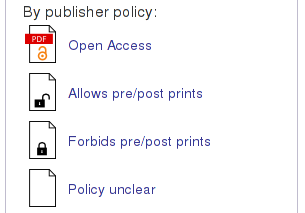
\includegraphics[scale=0.5]{img/policy.png}
\caption{Screenshot of the search criteria}
\end{figure}

\subsection{Full text availability}

Full text availability is detected by searching for the articles in open
repositories. Our goal is to detect only copies present in open
repositories, and not on personal homepages, to foster the use of
repositories. Incidentally, it is also much easier to discover
automatically a preprint when it is stored in an open repository.

The full text availability is presented with a symbol:

\begin{figure}[htbp]
\centering
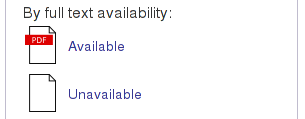
\includegraphics[scale=0.5]{img/availability.png}
\caption{Screenshot of the availability criteria}
\end{figure}

\subsection{Combination of the two criteria}

These two criteria can be visually combined to help researchers grasp
instantly the status of their publications, as in the following example:

\begin{figure}[htbp]
\centering
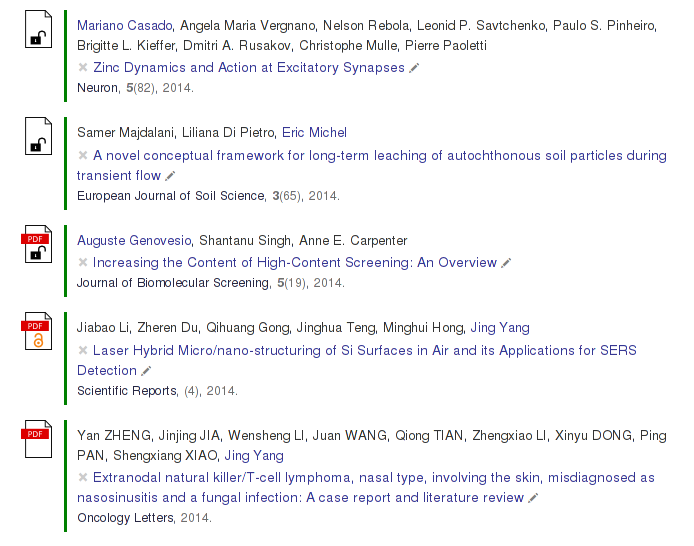
\includegraphics[scale=0.5]{img/publist.png}
\caption{Screenshot of the publications list}
\end{figure}

The two first papers were not found in any repository, but their
publisher's policy indicates that they could be made available. They
would then be marked as the third paper. The fourth paper is published
in an open access journal and is hence considered available. The last
paper is also available and the publisher policy is marked as unknown.

\section{Demo}

A prototype is running and encompasses some departments of the École
Normale Supérieure (ENS), a french university. It is online here:

\url{http://ens.dissem.in/}

The source code is released under the GNU General Public License version
2 or later, and can be found at:

\url{http://github.com/wetneb/dissemin}

\section{Technical details}

\subsection{Metadata sources}

We use two different tools to discover preprints:

\begin{itemize}
\item
  Our own OAI-PMH \cite{oaipmh} harvester, covering 8 millions of papers from the
  major open repositories such as arXiv, HAL and PubMed Central. The
  harvester acts as a proxy: it exposes the metadata it harvests as an
  OAI-PMH source, with additional metadata (OAI sets) to enable a search
  by author name. 
\item
  Bielefeld Academic Search Engine (through its API) \cite{lossau2006bielefeld}:
  this service covers a large collection of preprints, but the metadata it
  serves is not always very reliable, so we cannot afford to import
  systematically all the search results matching a given author in our
  database. However, if we have discovered a publication from another
  source and BASE can find a preprint for it, we mark this publication
  as available.
\item
  A CORE \cite{knoth2011core} interface is being implemented.
\end{itemize}

\subsection{Author disambiguation}

We perform automatic author name disambiguation to get accurate
publications list for each researcher. The problem can be formulated as
follows: given a list of researchers for each department in a
university, and given a list of millions of papers fetched from various
sources, find the papers corresponding to our known researchers. Our
approach is a two-stage algorithm, similar to the AuthorMagic heuristics
used in the Invenio platform \cite{weiler2011authormagic}.

\begin{itemize}
\item
  First, papers sharing a similar author name are grouped by similarity,
  so that two papers in the same group have most likely been authored by
  the same researcher.
\item
  Second, the relevance of each group of papers for our target
  researcher is estimated, and a cluster of similar papers is added to
  the publications list if the majority of these papers are considered
  relevant to the researcher.
\end{itemize}

Both steps use Support Vector Machines trained on one thousand manually
annotated papers.

\bibliographystyle{plain}
\bibliography{references}

\end{document}

